%*********************************************************%
% 17.11 : Alte Definitionen wieder hergestellt. (chaosbastler)
%*********************************************************
\subsection{Typen von Abbildungen}\label{kap_typabb}
\subsubsection{Definition}

\begin{figure}
\subfigure[surjektive
Abbildung]{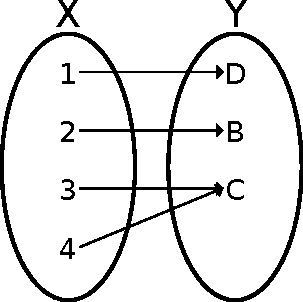
\includegraphics[width=3cm]{Surjection.pdf}}\hfill
\subfigure[injektive
Abbildung]{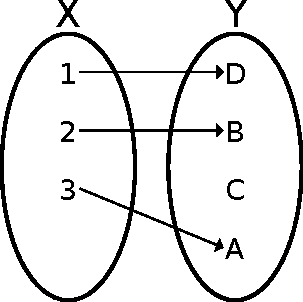
\includegraphics[width=3cm]{Injection.pdf}}\hfill
\subfigure[bijektive
Abbildungen]{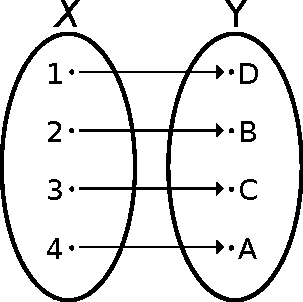
\includegraphics[width=3cm]{Bijection.pdf}}\hfill
\subfigure[identische
Abbildungen]{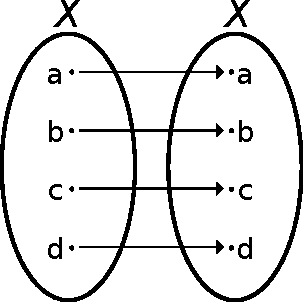
\includegraphics[width=3cm]{Identitaet.pdf}}
\end{figure}


Seinen A und B zwei Mengen und $f:{A}\longrightarrow{B}$ eine Abbildungsvorschrift.
Dann gibt es 3 besondere Typen von Abbildungen:
\begin{description}
\item[surjektive Abbildung] \emph{alle} Elemente von B mindestens einmal erfassen
$$ \forall b \in B \exists a \in A : f(a)=b $$
\item[injektive Abbildungen] alle Elemente von A erhalten \emph{unterschiedliche} Elemente aus B  (''keine Kollisionen``)
$$ \forall a_1,a_2  \in A : f(a_1)=f(a_2) \Rightarrow a_1 = a_2 $$
\item[bijektive Abbildungen] \emph{surjektiv und injektiv} zu gleich: alle A erhalten genau ein B und alle B werden getroffen.
Dies impliziert die Umkehrbarkeit der Funktion. Eine Sonderform der bijektiven
Abbildung ist die \emph{Identität}. Dabei wird jedes Element sich selbst zugeordnet.
$$ \forall b \in B \exists ! a \in A : f(a) = b $$
\end{description}

Ist $f \colon A \rightarrow B$ eine Abbildung, so sei für $X \subseteq A$ stets
$fX \coloneq f[X] \coloneq \{fx | x \in X\}$ die Menge der Bilder von $X$ unter
$f$.
Ferner heiße $\text{Bild}(f) = \text{Im}(f) \coloneq fA$ die
\emph{Bildmenge}\footnote{Bild = Image} von $f$. $f$ ist genau dann surjektiv,
wenn (gdw\footnote{im englischen Sprachraum \emph{iff} = if and only if}) $fA = B$
gilt, das heißt die Bildmenge von $f$ ist gleich der Zielmenge von $f$. Daraus
folgt: $fX \subseteq fA$

\newpage

\subsubsection{Bezeichnungen}
\begin{description}
\item Sind $A$ und $B$ Mengen, so bezeichnen $B^A \coloneq \text{Abb}(A,B)
\coloneq \Map(A,B)$ die Menge aller Abbildungen von $A$ nach $B$.
\item $\Surj(A,B)$ sei die Menge aller surjektiven Abbildungen
(\emph{Surjektionen}) von $A$ nach $B$,
\item $\Inj(A,B)$ sei die Menge aller injektiven Abbildungen
(\emph{Injektionen}) von $A$ nach $B$,
\item $\Bij(A,B)$ sei die Menge aller bijektiven Abbildungen
(\emph{Bijektionen}) von $A$ nach $B$.
\end{description}


\subsubsection{Mächtigkeit von Definitions- und Wertebereich}

Für Surjektionen gilt: $|A| \geq |B|$

Für Injektionen gilt: $|B| \geq |A|$

Weil für bijektive Abbildungen beide Aussagen gelten müssen gilt:
$$|A| \geq |B| \wedge |B| \geq |A| \Rightarrow |A| = |B| $$


Analog gilt auch:
$$ |A|<|B| \Longleftrightarrow \Surj(A,B) = \emptyset $$
$$ |A|>|B| \Longleftrightarrow \Inj(A,B) = \emptyset $$
$$ |A| \neq |B| \Longleftrightarrow \Bij(A,B) = \emptyset $$

Die ersten Aussagen schließen von einem Typ von Abbildung auf die Mächtigkeit von Definitions- und Wertebereich.
Die drei letzen Aussagen schließen von Definitions- und Wertebereich auf die (nicht) möglichen Typen von Abbildungen.

Würden die Beziehungen zwischen den Mächtigkeiten nicht gelten, würde z.B. die
Formel zur Mächtigkeit von $\Inj(A,B)$ zu Widersprüchen führen(vlg. nächstes
Kapitel).
